\subsection{When are random effects useful?}
\label{sec:whenrandomeffectsareuseful}

\subsubsection{Introduction to random effects}
\label{sec:introductiontorandomeffects}

(Generalised) Linear Mixed Models (GLMMs) are an extension of (Generalised) Linear Models (GLMs).
They add what are often called \textit{random effects} and \textit{mix} them with the normal predictors (\textit{fixed effects}) as used in GLMs.
Alternatively, statisticians speak of \textit{multilevel models} or \textit{hierarchical models} \citep{GelmanHill2006}, a terminology to be explained in Section~\ref{sec:hierarchicalormultilevelmodels}.

The purpose of including random effects is usually said to be the modeling of variance between groups of observations.
A single observation (alternatively \textit{data point}, \textit{measurement}, or \textit{unit}) is one atomic exemplar entering into the statistical analysis of a study.
In corpus linguistics, single observations can be understood as single lines in a concordance.
These concordance lines could contain, for example, clauses or sentences in which one of the alternants of a morpho-syntactic alternation occurs, the goal being to model the influence of diverse properties of the clauses or sentences on the choice of the alternants.
Along similar lines, they could contain occurrences of a contracted or a non-contracted form of words (like \textit{am} and \textit{'m} in English).
As another example, the concordance lines could contain NPs where two pre-nominal adjectives are used, the goal being to determine the factors influencing their relative ordering.
When such observations are grouped, it is often plausible to assume that there is some variance in the choice of the alternating forms or constructions at the group-level.
If this is the case and the grouping factor is not included in the model, the error terms within the groups will be correlated.
Put simply, this means that means of the group-wise errors vary.
Since the estimators used for estimating the parameters of GLMs work under the assumption of non-correlated errors, standard errors for model coefficients will typically be estimated as smaller than they nominally are, leading to increased Type I error rates in inferences about the coefficients.%
\footnote{Type I errors occur when the null hypothesis is rejected although it is true.
The requirement that error should be uncorrelated is often called ``independence (of errors)''.}
This gets even worse when there are within-group tendencies regarding the direction and strength of the influence of the other regressors, \ie when there is an interaction between them and the grouping factor (\eg \citealt{SchielzethForstmeier2009}).
This is why known variation by group should always be accounted for in the model.
Random effects are one convenient way to do so.

Groups can be defined by any linguistically relevant grouping factor, such as the individual speakers (or authors, writers, etc.), the regions where they were born or live, social groups with which they identify, but also time periods, genres, styles, etc.%
\footnote{Trivially, grouping factors should never be ordinal variables.
The are always categorical.}
Specific lexemes often have idiosyncratic affinities towards alternants in alternating constructions.
Therefore, exemplars containing specific lexemes also constitute groups.
In cases like the dative alternation in English, individual verbs co-occur with the alternants to different degrees.

The crucial question in specifying models is not whether to include these grouping factors at all, but rather whether to include them as fixed effects or as random effects.
Random effects structures are very suitable for accounting for group-level variation in regression, but while formulaic recommendations such as ``Always include random effects for speaker and genre!'' provide useful guidance for beginners, the choice between fixed and random effects can and should be made based on an analysis and understanding of the data set at hand and the differences and similarities in the resulting models.
The remainder of Section~\ref{sec:whenrandomeffectsareuseful} introduces three important points to consider about the structure of the data typically used in mixed modeling.
Then, Section~\ref{sec:modelspecificationandmodelingassumptions} provides a moderately technical introduction to modeling.
Section~\ref{sec:practicalguidewithr} shows how a mixed model is implemented in \texttt{R}.


\subsubsection{Crossed and nested effects}
\label{sec:crossedandnestedeffects}

\begin{table}
  \centering
  \begin{tabular}{lll}
    \toprule
    \textbf{Exemplar} & \textbf{Speaker}  & \textbf{Region}        \\
    \midrule
                    1 &           Daryl  &         Tyneside       \\
                    2 &           Daryl  &         Tyneside       \\
                    3 &           Riley  &         Tyneside       \\
                    4 &           Riley  &         Tyneside       \\
                    5 &           Dale   &         Greater London \\
                    6 &           Dale   &         Greater London \\
                    7 &           Reed   &         Greater London \\
                    8 &           Reed   &         Greater London \\
    \bottomrule
  \end{tabular}
  \caption{Illustration of nested factors}
  \label{tab:nested}
\end{table}

This section discusses a distinction that arises when there is more than one grouping factor.
When this is the case, each pair of grouping factors can be \textit{nested} or \textit{crossed}.
By way of example, we can group exemplars (such as sentences) by the individual speakers who wrote or uttered them, and we can group speakers by their region of birth.
Such a data set would intrinsically be \textit{nested}, as Table~\ref{tab:crossed} illustrates.
Since speakers have a unique region of birth, Tyneside is the unique \textit{region} value for the speakers Daryl and Riley, and Greater London is the unique \textit{region} value for Dale and Reed.
In this example, the region factor nests the speaker factor.
This example was chosen because the nesting is conceptually necessary.
However, even when a data set has a nested structure by accident, standard packages in \texttt{R} will also treat them as nested (see Section~\ref{sec:specifyingmodelsusinglme4inr}).

When the grouped entities (themselves groups) do not uniquely belong to levels of the grouping factor, the factors are \textit{crossed}.
Continuing the example, crossed factors for speaker and mode are illustrated in Table~\ref{tab:crossed}.
%
\begin{table}
  \centering
  \begin{tabular}{lll}
    \toprule
    \textbf{Exemplar} & \textbf{Speaker}  & \textbf{Mode}   \\
    \midrule
                    1 &           Daryl  &         Spoken  \\
                    2 &           Daryl  &         Written \\
                    3 &           Riley  &         Spoken  \\
                    4 &           Riley  &         Spoken  \\
                    5 &           Dale   &         Written \\
                    6 &           Dale   &         Written \\
                    7 &           Reed   &         Spoken  \\
                    8 &           Reed   &         Written \\
    \bottomrule
  \end{tabular}
  \caption{Illustration of crossed factors}
  \label{tab:crossed}
\end{table}
%
While there are only spoken sentences by Riley and only written sentences by Dale in the sample, there is one spoken and one written sentence each by Daryl and Reed.
There is a many-to-many relation between speakers and modes, which is characteristic of crossed factors.
In Table~\ref{tab:nested}, the relation between speakers and regions is many-to-one, which is typical of nested factors.

With more than two grouping factors, there can be more than one level of nesting.
Mode could nest genre if genres are defined such that each genre is either exclusively spoken or written.
Similarly, in a study on adjectives we might want to describe adjectives as being either intersective or non-intersective.
Within the two groups, a finer-grained semantic classification might be nested, which itself nests single adjective lexemes.
However, not all of these structures should be modeled as nested random effects.
In the latter case, for example, the low number of levels in one factor (intersectivity with just two levels) predestines it as a second-level predictor rather than a nesting factor; see Section~\ref{sec:hierarchicalormultilevelmodels}.

\subsubsection{Hierarchical or multilevel modeling}
\label{sec:hierarchicalormultilevelmodels}

This section describes the types of data to be used in true multilevel models.
Let us assume that we wanted to account for lexeme-specific variation in a study on an alternation phenomenon such as the dative alternation in English by specifying the lexeme as a random effect in the model.
Additionally, we suspect or know that a lexeme's overall frequency influences its preferences for occurring in the construction alternants.
A similar situation would arise in a study of learner corpus data (even of the same alternation phenomenon) with a learner grouping factor if we also knew that the number of years learners have learned a language influences their performance with regard to a specific phenomenon.
In such cases, variables like \textit{frequency} and \textit{number of learning years} are constant for each level of the grouping factor (\textit{lexeme} and \textit{learner}, respectively).
In other words, each lexeme has exactly one overall frequency, and each learner has had a fixed number of years of learning the language.

\begin{table}
  \centering
  \begin{tabular}{llllll}
    \toprule
    \multicolumn{3}{l}{\textbf{Level of observations}}          & \multicolumn{2}{l}{\textbf{Group level}}  & \textbf{Outcome} \\
    \textbf{Exemplar} & \textbf{Givenness} & \textbf{NP length} & \textbf{Verb} & \textbf{Verb freq.}       & \textbf{Alternant}\\
    \midrule
            1 &     New   &      8    &    give   &   6.99   & 1 \\
            2 &     Old   &      7    &    give   &   6.99   & 1 \\
            3 &     Old   &      5    &    give   &   6.99   & 2 \\
            4 &     Old   &      5    &    grant  &   5.97   & 2 \\
            5 &     New   &      9    &    grant  &   5.97   & 1 \\
            6 &     Old   &      6    &    grant  &   5.97   & 2 \\
            7 &     New   &      11   &   promise &   5.86   & 2 \\
            8 &     New   &      10   &   promise &   5.86   & 1 \\
            9 &     Old   &      9    &   promise &   5.86   & 2 \\
    \bottomrule
  \end{tabular}
  \caption{Illustration of a fictional data set which requires multilevel modeling; NP length could be measured in words; the lemma frequencies are actual logarithm-transformed frequencies per one million tokens taken from ENCOW14A \citep{SchaeferBildhauer2012}; the outcome column encodes whether alternant 1 or 2 was chosen}
  \label{tab:multilevel}
\end{table}

Such variables are thus interpretable only at the group-level.
Table~\ref{tab:multilevel} illustrates such a data set (fictional in this case).
It might be a small fraction of the data used to predict whether a ditransitive verb is used in the dative shift construction or not.
The givenness and the NP length status vary at the level of observations.
To capture verb lemma specific tendencies, a verb lemma grouping factor is added.
The verb lemma frequency necessarily varies at the group level because each lemma has a unique frequency.
In such cases, an adequately specified multilevel model uses the group-level variables to partially predict the tendency of the grouping factor.
Put differently, the idiosyncratic effect associated with a lexeme, speaker, genre, etc.\ is split up into a truly idiosyncratic preference and a preference predictable from group-level variables.
This is achieved by specifying a second (linear) model which predicts the group-level random effect itself.
Such second-level models can even contain modeled effects themselves, giving rise to third-level models, and so on.
The data look similar to multilevel nesting, but (i) second-level models can account for continuous numerical predictors at the group-level, which nesting cannot, and (ii) there might be situations where specifying even categorical second-level grouping factors as fixed effects in a second-level model is more appropriate than adding nested random effects (see Section~\ref{sec:modelspecificationandmodelingassumptions}).

As in the case of nested vs.\ crossed factors, standard packages in \texttt{R} usually take care of hierarchical modeling automatically, given that the data are structured appropriately.
This might, however, lead to situations where practitioners specify multilevel models without even knowing it, which in turn can lead to misinterpretations of the results.

\subsubsection{Random slopes as interactions}
\label{sec:randominterceptsandslopes}

This section introduces the data patterns that gives rise to \textit{varying intercepts} and \textit{varying slopes}. 
Varying intercepts are an adequate modeling tool when the overall tendency in the outcome variable changes with the levels of the grouping factor.

\begin{figure}[!htpb]
  \centering
  \includegraphics[width=0.5\textwidth]{graphics/var_int}~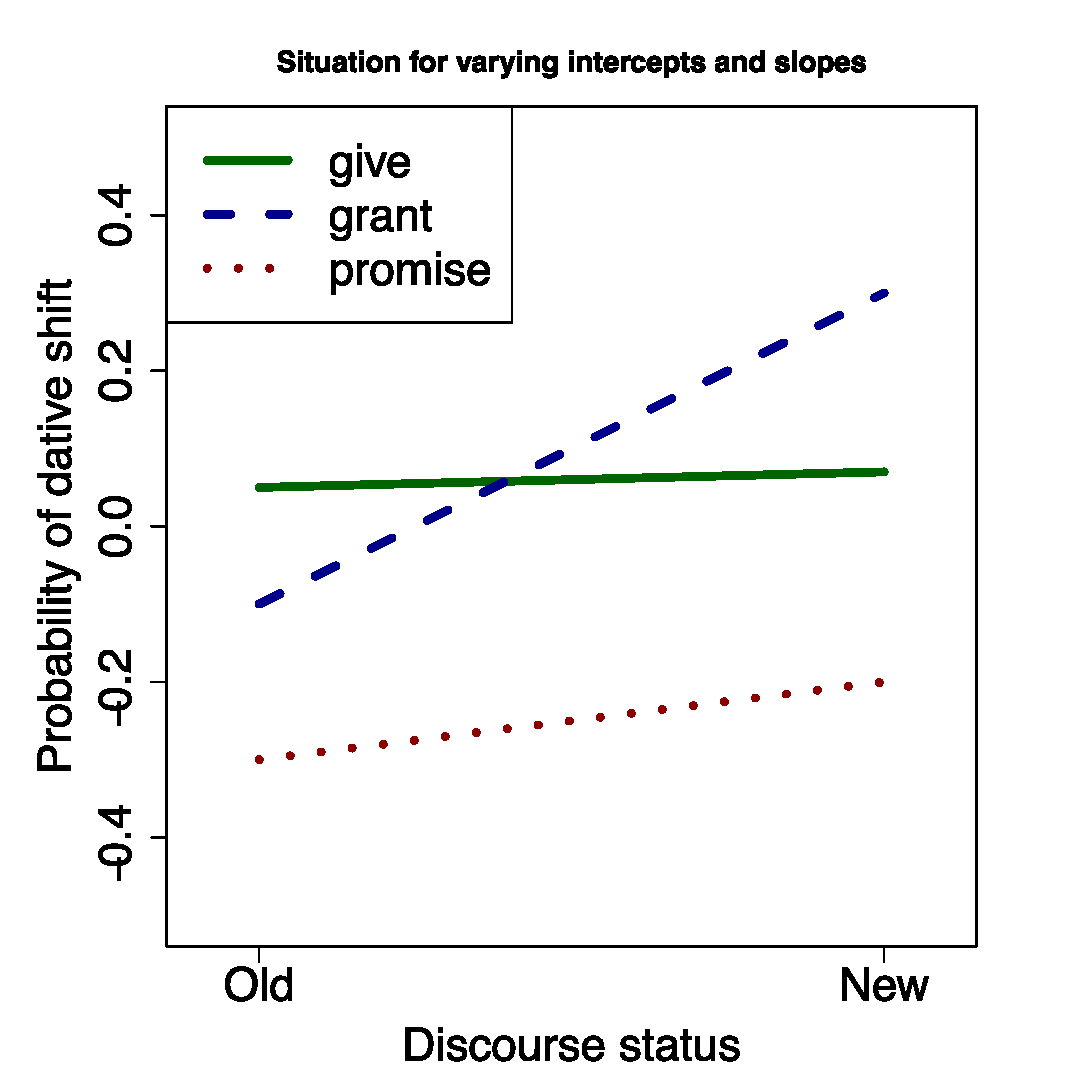
\includegraphics[width=0.5\textwidth]{graphics/var_int_slope}
  \caption{Interaction plots of fictional data in situations for varying intercepts or varying intercepts and additional varying slopes}
  \label{fig:varintlsope}
\end{figure}

We assume that we are looking at an alternation phenomenon like the dative alternation, wherein we are interested in the probability that, under given circumstances, the dative shift construction is chosen.
In the examination of the data, it turns out that the probability of the dative shift changes for \textit{old} and \textit{new} dative NPs.
The verb lemma also influences the probability of either variant being used.
The situation can now be as in the left or the right panel of Figure~\ref{fig:varintlsope}.
In the situation depicted in the left panel, the overall level in probability changes with the verb lemma, but for each verb lemma, the values change roughly by the same amount in exemplars with old and new dative NPs.
Note that the lines are not perfectly parallel because the figure is supposed to be an illustration of a data set rather than a fitted model, and we always expect some chance variation in data sets.
In the situation depicted in the right panel, however, the overall levels are also different between lemmas, but additionally the lemma-specific tendencies also vary between exemplars with old and new NPs.
This is in fact nothing but an interaction between two factors (verb lemma and givenness), and we could use a fixed-effect interaction to take it into account.
However, if the verb lemma factor is used as a random effect grouping factor, the interaction is modeled as a so-called \textit{random slope}.
In the next section, it is shown how all the different types of data sets discussed so far can be modeled using fixed effects models or, alternatively, using mixed effects models.
Which one is more appropriate will be argued to be better understood as a technical rather than a conceptual question.

